\documentclass{beamer}


\usepackage[utf8]{inputenc}
\usepackage{lmodern} 
\usepackage[utf8]{inputenc}
\usepackage{lmodern} 
\usepackage{listings}
\usepackage{xcolor} 
\usepackage{graphicx}

\lstset{
	language=C,
	basicstyle=\ttfamily\small,
	keywordstyle=\color{blue},
	commentstyle=\color{green},
	stringstyle=\color{red},
	breaklines=true,
	breakatwhitespace=true,
	showstringspaces=false,
	frame=single,
	morekeywords={import, as, from, ctypes, numpy, matplotlib, pyplot, None},
	xleftmargin=0pt,
	framexleftmargin=0pt,
	aboveskip=0pt,
	belowskip=0pt
}




\definecolor{myblue}{RGB}{48, 63, 159}

\setbeamercolor{palette primary}{bg=myblue, fg=white}
\setbeamercolor{structure}{fg=myblue}
\setbeamercolor{frametitle}{bg=myblue, fg=white}
\setbeamercolor{title}{bg=myblue, fg=white}
\setbeamercolor{footlinecolor}{bg=myblue, fg=white}


\defbeamertemplate*{title page}{mytemplate}{
	\vfill
	\begin{center}

		\begin{beamercolorbox}[wd=0.8\paperwidth, center, rounded=true, shadow=true]{title}
			\usebeamerfont{title}\inserttitle\par
		\end{beamercolorbox}
		\vspace{2cm} 

		\usebeamerfont{author}\insertauthor
		\vspace{1cm} 
		\usebeamerfont{date}\insertdate
	\end{center}
	\vfill
}


\defbeamertemplate*{frametitle}{mytemplate}{
	\begin{beamercolorbox}[wd=\paperwidth, ht=2.5ex, dp=1.5ex, left]{frametitle}
		\hspace{1em}\usebeamerfont{frametitle}\insertframetitle
	\end{beamercolorbox}
}


\setbeamertemplate{footline}{
	\begin{beamercolorbox}[wd=\paperwidth, ht=2.25ex, dp=1ex]{footlinecolor}
		\hspace{1em}\usebeamerfont{author in footline}\insertshortauthor
		\hfill
		\usebeamerfont{title in footline}\insertshorttitle
		\hfill
		\usebeamerfont{date in footline}\insertdate \hspace{1em} \insertframenumber/\inserttotalframenumber \hspace{0.5em}
	\end{beamercolorbox}
}


\setbeamerfont{author in footline}{size=\tiny}
\setbeamerfont{title in footline}{size=\tiny}
\setbeamerfont{date in footline}{size=\tiny}



\title{1.6.3}
\author{Shriyansh Chawda-EE25BTECH11052}
\date{August 23, 2025}



\begin{document}
	

		\setbeamertemplate{footline}{} 
		\frame{\titlepage}
	
	
	

	\begin{frame}{Question} 
			Determine if the points (1, 5), (2, 3) and (-2, -11) are collinear.
	\end{frame}
	
	

	\begin{frame}{Solution}

Points $\mathbf{A}, \mathbf{B}, \mathbf{C}$ are defined to be collinear if
\[ \text{rank}\big(\mathbf{B}-\mathbf{A} \;\;\; \mathbf{C}-\mathbf{A}\big) = 1 \tag{1.1.9.1}\]
	
	Let $\mathbf{A}=(1,5),\ \mathbf{B}=(2,3),\ \mathbf{C}=(-2,-11)$.
	From this, the collinearity matrix can be expressed as
	\[
	\left(
	\begin{array}{cc}
		\mathbf{B}-\mathbf{A} & \mathbf{C}-\mathbf{A}
	\end{array}
	\right)
	=
	\begin{pmatrix}
		1 & -3\\
		-2 & -16
	\end{pmatrix}
	\ \overset{R_2\leftarrow R_2+2R_1}{\longrightarrow}\
	\begin{pmatrix}
		1 & -3\\
		0 & -22
	\end{pmatrix}
	\]
	which is a rank $2$ matrix. Using (1.1.9.1), the above-mentioned property,
	we conclude that the given points are \textbf{not} collinear.
	
	\end{frame}

\begin{frame}[fragile]{C Code - Collinearity Formula}
	\begin{lstlisting}
#include <math.h>

// Return 1 if collinear, 0 otherwise
int check_collinearity(double x1, double y1,
double x2, double y2,
double x3, double y3,
double tol)
{
	double det = (x2 - x1) * (y3 - y1) - (y2 - y1) * (x3 - x1);
	return fabs(det) <= tol ? 1 : 0;
}
	
	\end{lstlisting}
\end{frame}

\begin{frame}[fragile,plain]{Python Code}
	\begin{lstlisting}[language=Python]
import ctypes
import matplotlib as mp
import matplotlib.pyplot as plt
import numpy as np


lib = ctypes.CDLL('./libcollinearity.so')
lib.check_collinearity.argtypes = [ctypes.c_double, ctypes.c_double,
ctypes.c_double, ctypes.c_double,
ctypes.c_double, ctypes.c_double,
ctypes.c_double]
lib.check_collinearity.restype = ctypes.c_int

def check_collinearity(A, B, C, tol=1e-9):
return lib.check_collinearity(A[0], A[1], B[0], B[1], C[0], C[1], tol)

	\end{lstlisting}
\end{frame}


\begin{frame}[fragile,plain]{Python Code}
\begin{lstlisting}[language=Python]
A = (1,5)
B = (2,3)
C = (-2,-11)

is_collinear = check_collinearity(A, B, C)
print("Collinear" if is_collinear else "Not collinear")


plt.figure(figsize=(8, 8))


x_line = np.linspace(min(A[0], C[0]) - 1, max(A[0], C[0]) + 1, 100)
slope = (C[1] - A[1]) / (C[0] - A[0])
y_line = A[1] + slope * (x_line - A[0])
plt.plot(x_line, y_line, 'k--', label="Line through A & C")
	
\end{lstlisting}
\end{frame}

\begin{frame}[fragile,plain]{Python Code}
	\begin{lstlisting}[language=Python]
plt.plot(A[0], A[1], 'ro', label='A')
plt.plot(B[0], B[1], 'go', label='B')
plt.plot(C[0], C[1], 'bo', label='C')

plt.text(A[0]+0.2, A[1], f"A{A}", fontsize=12)
plt.text(B[0]+0.2, B[1], f"B{B}", fontsize=12)
plt.text(C[0]+0.2, C[1], f"C{C}", fontsize=12)

mp.use("TkAgg")
plt.xlabel('x')
plt.ylabel('y')
plt.title('Collinearity Check')
plt.legend()
plt.grid(True)
plt.gca().set_aspect('equal', adjustable='box')


	\end{lstlisting}
\end{frame}

\begin{frame}[fragile,plain]{Python Code}
	\begin{lstlisting}[language=Python]
plt.savefig(
"/home/shriyasnh/Desktop/matgeo/1.6.3/codes",
dpi=300,
bbox_inches='tight'
)
plt.show()
	\end{lstlisting}
\end{frame}

\begin{frame}

	\begin{figure}[H]
		\centering
		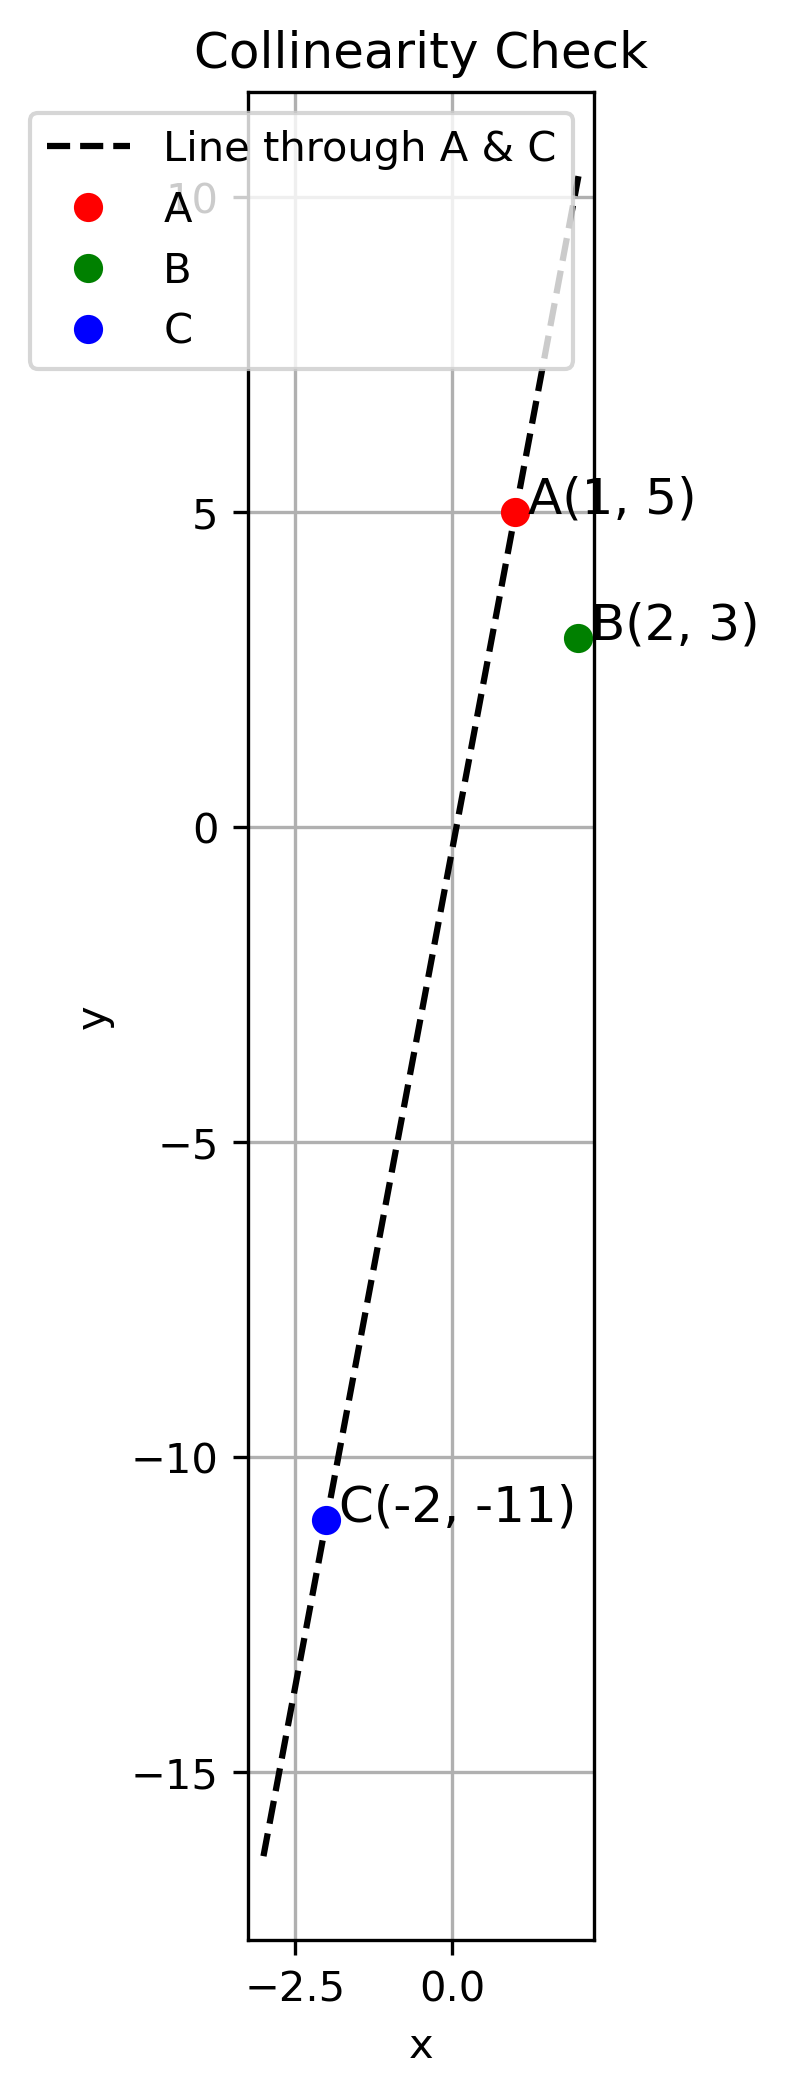
\includegraphics[width=0.3\linewidth]{figs/collinearity}
		\caption{}
		\label{fig:collinearity}
	\end{figure}
	
\end{frame}




\end{document}